\chapter{Présentation du projet}

		Le taquin est un jeu de puzzle, constitué d’un rectangle dans lequel se trouve des cases. Ces cases contenant des lettres de l'alphabet,
		des nombres ou encore des morceaux d’images, peuvent glisser les unes sur les autres. Parmi les cases, l’une d'entre elles est vide.
		Le but du jeu du taquin consiste à reconstituer le puzzle en formant une image (lorsque les cases forment une image) ou de ranger les nombres par ordre croissant (lorsque les cases contiennent des nombres) en glissant l'un des éléments contigus à la case vide vers celle-ci. Avec l’interface graphique, l'utilisateur a la possibilité de choisir sa propre image pour le taquin qu’il devra reconstituer.

		Le but de ce devoir a été de réaliser un taquin sous forme d’une application de jeu, dotée d'une interface graphique, tout en pouvant être utilisée sans interface graphique c'est-à-dire être jouable en ligne de commande. L'application a été intégralement réalisée avec le design pattern MVC, avec un modèle totalement indépendant de l'interface graphique.

		\begin{figure}[H]
			\centering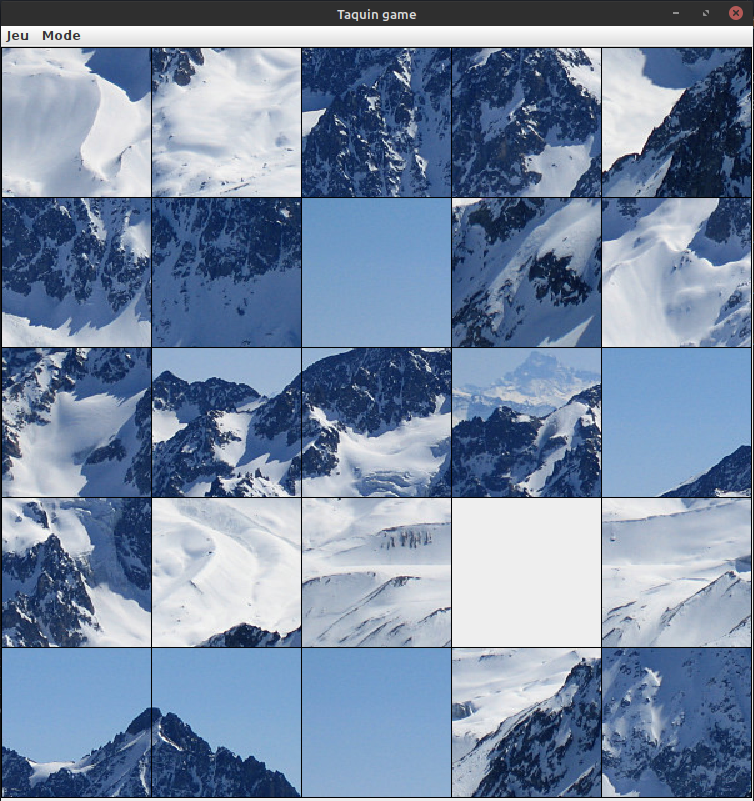
\includegraphics[width=0.30\textwidth, keepaspectratio]{img/jeuImage.png}
			\caption{Image du jeu avec le mode Image}
			\label{fig:JeuImage}
		\end{figure}

		\begin{figure}[H]
			\centering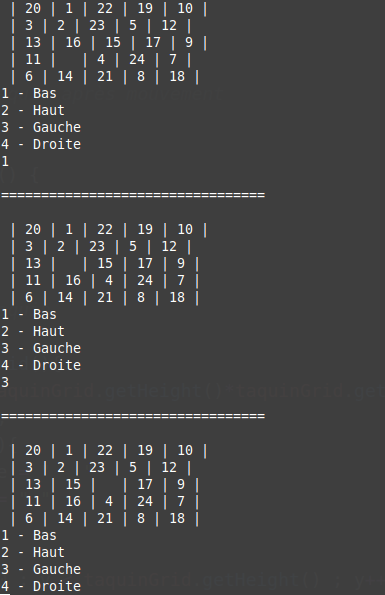
\includegraphics[width=0.30\textwidth, keepaspectratio]{img/jeuConsole.png}
			\caption{Image du jeu en console}
			\label{fig:JeuConsole}
		\end{figure}
